\documentclass[letterpaper]{article}
\usepackage[utf8]{inputenc}
\usepackage[parfill]{parskip}    % Activate to begin paragraphs with an empty line rather than an indent
\usepackage{graphicx}
\usepackage{amssymb}
\usepackage{amsmath}
\usepackage{amsthm}
\usepackage{mathtools}

\usepackage{afterpage}

\usepackage{algorithm}
\usepackage{algpseudocode}

\usepackage{verse}

\newtheorem{theorem}{Theorem}[section]
\newtheorem{corollary}{Corollary}[theorem]
\newtheorem{lemma}[theorem]{Lemma}

\theoremstyle{remark}
\newtheorem*{remark}{Remark}

\usepackage{epstopdf}
\usepackage{circuitikz}
\usepackage[separate-uncertainty = true,multi-part-units=single]{siunitx}
\usepackage{booktabs}
\usepackage{enumitem}
\usepackage[toc,page]{appendix}
\usepackage{color}
\usepackage{pgfplots}
\usepackage{pgfplotstable}
\usepackage{caption}
\usepackage{subcaption}
\usepackage{url}
\usepackage{multirow}
\usepackage{makecell}
\usepackage[round]{natbib}   % omit 'round' option if you prefer square brackets
\usepackage{titling}
\usepackage{siunitx}

\usepackage{setspace}
% \doublespacing
\usepackage{float}


\pgfplotsset{compat=1.14}

%  Special math symbols
%       floor, ceiling, angled brackets
%-----------------------------------------------------------------------
\newcommand{\floor}[1]{\left\lfloor #1\right\rfloor}
\newcommand{\ceil}[1]{\left\lceil #1\right\rceil}
\newcommand{\etal}{\textit{et al.}}
\newcommand{\RE}{\mathbb{R}}        % real space
\newcommand{\ZZ}{\mathbb{Z}}        % integers
\newcommand{\NN}{\mathbb{N}}        % natural numbers
\newcommand{\eps}{{\varepsilon}}    % prettier epsilon
%-----------------------------------------------------------------------
%  Tighter lists
%-----------------------------------------------------------------------
\newenvironment{itemize*}% Tighter itemized list
  {\begin{itemize}%
    \setlength{\itemsep}{-0.5ex}%
    \setlength{\parsep}{0pt}}%
  {\end{itemize}}
\newenvironment{description*}% Tighter description list
  {\begin{description}%
    \setlength{\itemsep}{-0.5ex}%
    \setlength{\parsep}{0pt}}%
  {\end{description}}
\newenvironment{enumerate*}% Tighter enumerated list
  {\begin{enumerate}%
    \setlength{\itemsep}{-0.5ex}%
    \setlength{\parsep}{0pt}}%
  {\end{enumerate}}
%-----------------------------------------------------------------------
% Typing shortcuts
%-----------------------------------------------------------------------
\newcommand{\X}{\mathbb{X}}
\newcommand{\SG}{\mathbf{S}}
\newcommand{\GE}{\mathcal{G}}
\newcommand{\ST}{\,:\,}
\renewcommand{\tilde}[1]{\widetilde{#1}}
\newcommand{\diam}{\mathrm{diam}}
\newcommand{\sq}{\square}
\newcommand{\half}[1]{\frac{#1}{2}}
\newcommand{\inv}[1]{\frac{1}{#1}}
\newcommand{\alg}{\textsf{SplitReduce}}
\newcommand{\sz}[1]{\sigma_{#1}}
\newcommand{\LL}{\mathcal{L}}
\newcommand{\softOmega}{\widetilde{\Omega}} 
\newcommand{\softO}{\widetilde{O}}
\newcommand{\OO}{O^*}  %or \widetilde{O}?

\newcommand{\norm}[1]{\left\lVert#1\right\rVert}

\newcommand{\dx}{\mathrm{d}x}
\newcommand{\dy}{\mathrm{d}y}
\newcommand{\dz}{\mathrm{d}z}
\newcommand{\dt}{\mathrm{d}t}
\newcommand{\du}{\mathrm{d}u}
\newcommand{\dtheta}{\mathrm{d}\theta}
\newcommand{\dq}{\mathrm{d}q}
\newcommand{\diff}{\mathrm{d}}
\newcommand{\dV}{\mathrm{d}V}
\newcommand{\dL}{\mathrm{d}L}
\newcommand{\dA}{\mathrm{d}A}
\newcommand{\dH}{\mathrm{d}H}
\newcommand{\df}{\mathrm{d}f}
\newcommand{\dg}{\mathrm{d}g}
\newcommand{\dr}{\mathrm{d}r}
\newcommand{\dw}{\mathrm{d}w}
\newcommand{\dv}{\mathrm{d}v}
\newcommand{\dI}{\mathrm{d}I}

\newcommand*\len[1]{\overline{#1}}

\DeclarePairedDelimiter\abs{\lvert}{\rvert}%

\newcommand\note[1]{\marginpar{\textcolor{red}{#1}}}
\newcommand*{\tageq}{\refstepcounter{equation}\tag{\theequation}}

\newcommand*{\equals}{=}

\usepackage{fancyhdr}

\pgfplotscreateplotcyclelist{grayscale}{
    thick,white!10!black,mark=x,mark options=solid, dashed\\%
    thick,white!20!black,mark=o,mark options=solid\\%
}

\newcommand{\mat}[1]{\ensuremath{\begin{bmatrix}#1\end{bmatrix}}}
\newcommand{\eqn}[1]{\begin{alignat*}{2}#1\end{alignat*}}
\newcommand{\p}[2]{\frac{\partial #1}{\partial #2}}
\newcommand*{\thus}{&\implies\quad&}

\newcommand{\answer}[1]{\framebox{$\displaystyle #1 $}}

 
\pagestyle{fancy}
\fancyhf{}
\rhead{Rahul Arya}
\lhead{EE 16B}
\cfoot{\thepage}

\title{Lecture 7 - Notes}
\author{Rahul Arya}
\date{February 2019}
\begin{document}

\maketitle

\section{Overview}
Using the method of phasors, we now know how to systematically analyze circuits consisting of inductors, capacitors, and resistors that are powered by sinusoidal voltage and current sources. Here, we will discuss some mathematical techniques that make such analysis easier, and look at how to interpret the results of our analysis.

\section{Complex Numbers}
Recall that a complex number $z$ can be uniquely written as
\[
    z = a + bj,
\]
where $a$ and $b$ are both real numbers. Recall also that the magnitude of $z$ is defined to be
\[
    \abs{z} = z\overline{z} = a^2 + b^2.
\]
We can plot complex numbers on a 2D plane, known as the \emph{complex plane}\footnote{Or an ``Argand Diagram'' if simple naming conventions aren't your thing.} as follows:
\begin{center}
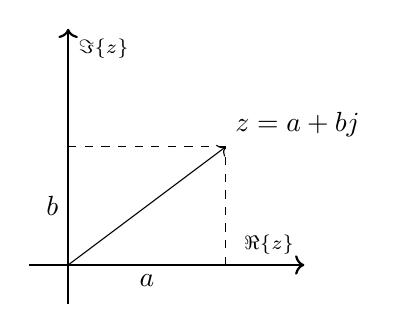
\begin{tikzpicture}
    \begin{scope}[thick,font=\scriptsize]
    \draw [->] (-0.5,0) -- (3,0) node [above left]  {$\Re\{z\}$};
    \draw [->] (0,-0.5) -- (0,3) node [below right] {$\Im\{z\}$};
    \end{scope}
    \draw [->] (0, 0) -- (2, 1.5);
    \draw[dashed] (2, 0) to (2, 1.5);
    \draw[dashed] (0, 1.5) to (2, 1.5);
    \draw (0, 0.75) node[left] {$b$};
    \draw (1, 0) node[below] {$a$};
    \draw (2, 1.5) node[above right] {$z = a + bj$};
\end{tikzpicture}
\end{center}
On this plane, we can view each complex number $z$ as a vector. By the Pythagorean Theorem, the length of the vector $z$ equals $\abs{z}$, which is clear visually.

Note that the angle $\theta$ that $z$ makes with the $x-axis$ satisfies the properties that
\eqn{
    && \sin{\theta} &= \frac{b}{\abs{z}} \\
    && \cos{\theta} &= \frac{a}{\abs{z}} \\
    && \tan{\theta} &= \frac{b}{a}. \\
}
Using trigonometric inverses, we can easily reconstruct $\theta$ from the components of $z$.

Now, observe that we can rewrite $z$ as follows:
\eqn{
    && z &= a + bj \\
    &&&= \abs{z}\cos{\theta} + \abs{z}\sin{\theta}b j \\
    &&&= \abs{z} \left(\cos{\theta} + j \sin{\theta} \right) \\
    &&&= \abs{z} e^{j\theta},
}
using Euler's formula for the last simplification. This new way of writing complex numbers is known as the \emph{polar form}, and makes multiplying and dividing complex numbers very easy. Note that we often refer to the angle $\theta$ of a complex number $z$ as $\angle z$, and refer to it verbally as the \emph{argument} of $z$.

From the polar form, we immediately obtain the following identities, which we will present without proof:
\eqn{
    && \angle z^k &= k\angle z \\
    && \angle \frac{1}{z} &= -\angle z \\
    && k\angle z &= \angle z,
}
where $k \in \mathbb{R}$ and $z \in \mathbb{C}$. These identities will prove useful shortly.

\section{Circuit Example and Transfer Functions}
Consider the circuit:
\begin{center}
\begin{circuitikz}[american]
\draw (0, 0) node[ground] {} to[sinusoidal voltage source, l=$V_0\cos{\omega t}$, v<=$ $] (0, 4) to (2, 4) to[R, l=$R$] (2, 2) node[ocirc] {} node[right] {$u(t)$} to[C, l=$C$] (2, 0) to (0, 0);
\end{circuitikz}
\end{center}
Notice that this circuit is very similar to a voltage divider, except that one resistor has been replaced by a capacitor. As we discussed last lecture, we can still apply our standard circuit analysis techniques on the phasors representing the voltages and currents in this system.

We saw last time that the input voltage phasor was
\[
    \tilde{V} = V_0.
\]
Applying the equation for a voltage divider, we find the voltage phasor at $u(t)$ to be
\[
    \tilde{u} = \frac{R}{R + \frac{1}{j\omega C}}\tilde{V}.
\]

We won't substitute in our known value for $\tilde{V}$ just yet. We define the coefficient for $\tilde{V}$ to be the \emph{transfer function}
\[
    H(\omega) = \frac{\frac{1}{j\omega C}}{R + \frac{1}{j\omega C}}.
\]
More broadly, transfer functions map an angular frequency $\omega$ to a ratio of two phasors - an input and an output - and are used to characterize the behavior of a system acrss a range of frequencies. Here, our transfer function relates two voltage phasors, but they can also relate two current phasors, or a voltage phasor with a current phasor, in a similar manner.

Observe that as transfer functions are the ratio of two phasors, they are complex-valued in general. Thus, we can write
\[
    H(\omega) = M(\omega) e^{j \theta},
\]
where $M(\omega)$ is the magnitude of the transfer function, and $\theta$ is its argument.

In this example, we may rearrange $H(\omega)$ to become
\eqn{
    && H(\omega) &= \frac{\frac{1}{j\omega C}}{R + \frac{1}{j\omega C}} \\
    &&&= \frac{1}{1 + j\omega RC} \\
    &&&= \frac{1 - j\omega RC}{1 + \omega^2R^2C^2} \\
    &&&= \frac{1}{\omega^2R^2C^2} (1 - j\omega RC).
}
Thus, since the coefficient at the front is real, we find that
\[
    \theta = \angle H(\omega) = \angle(1 - j\omega RC) = -\tan^{-1}(\omega RC).
\]
We can also compute the magnitude of $H$
\[
    M(\omega) = \abs{H(\omega)} = \frac{1}{\sqrt{1 + \omega^2 R^2C^2}},
\]
using the fact that $\abs{1/z} = 1 / \abs{z}$.

Now, we can multiply through with $\tilde{V}$, to compute the voltage phasor $\tilde{u}$
\eqn{
    && \tilde{u} &= H(\omega) \tilde{v} \\
    &&&= M(\omega) e^{j\omega} V_0 \\
    &&&= \frac{V_0}{\sqrt{1 + \omega^2R^2C^2}} e^{j\omega}.
}
Solving for $u(t)$,
\eqn{
    && u(t) &= \frac{1}{2} \left( \tilde{u}e^{j\omega t} + \overline{\tilde{u}}e^{-j\omega t} \right) \\
    &&&= \frac{1}{2} \left(V_0M(\omega) e^{j\theta} e^{j\omega t} + V_0M(\omega) e^{-j\theta} e^{-j\omega t} \right) \\
    &&&= \frac{1}{2} \left(V_0M(\omega) e^{j(\theta + \omega t)} + V_0M(\omega) e^{-j(\theta + \omega t)} \right) \\
    &&&= M(\omega) V_0 \cos{(\omega t + \theta)},
}
which can be expressed using our solution for $H$ as
\[
    u(t) = \frac{V_0}{\sqrt{1 + \omega^2 R^2C^2}} \cos{(\omega t -\tan^{-1}(\omega RC))}.
\]
We see here that the transfer function will scale the input signal by a factor of $M(\omega)$, and shift its phase by an angle $\theta$. It can be easily shown that this property of transfer functions holds true for arbitrary sinusoidal input voltages, though we will not do so here.

Thus, we can follow the following procedure when analyzing a circuit accepting a range of unknown input signals:
% \begin{itemize}
%     \item Convert all the initial voltage and current sources into phasors.
%     \item Calculate the output voltage and current phasors using the known impedances of the circuit components.
%     \item Compute the desired output values in the time domain.
% \end{itemize}

% Or if we're interested in knowing the behavior of a circuit for a range of inputs, we can:
\begin{itemize}
    \item Express the unknown input current or voltage as phasors.
    \item Solve for the output voltage and current phasors as functions of the input phasors, and so determine the transfer function.
    \item Look at the magnitude and phase shift of the transfer function at the input frequency to determine the behavior of the circuit.
\end{itemize}

% The latter procedure is most useful when considering a class of circuits known as \emph{filters}, which remove certain undesired components from a signal. 

\section{Series and Parallel Rules for Impedances}
Notice, in particular, that $M(\omega)$ goes to zero as $\omega \to \infty$, but remains close to $1$ when $\omega \approx 0$. We saw similar behavior at a qualitative level when we looked at series and parallel approximate impedances, but here we are able to derive the behavior more rigorously. In particular, we will attempt to justify that the rules stating that
\[
    |\tilde{Z_1} + \tilde{Z_2}| \approx \max{(\tilde{Z_1}, \tilde{Z_2})}
\]
and
\[
    |(\tilde{Z_1} || \tilde{Z_2})| \approx \min{(\tilde{Z_1}, \tilde{Z_2})}
\]
still hold, even when dealing with complex impedances. Notice that these series and parallel rules are essentially combining two transfer functions (the impedances $\tilde{Z_1}$ and $\tilde{Z_2}$) to produce a new transfer function. We will now present some additional intuition for these rules, though we will not prove them fully rigorously.

For the series case, imagine plotting $\tilde{Z_1}$, $\tilde{Z_2}$, and $\tilde{Z_1 + Z_2}$ on the complex plane:
\begin{center}
\begin{tikzpicture}
    \begin{scope}[thick,font=\scriptsize]
    \draw [->] (-1,0) -- (6,0) node [above left]  {$\Re\{z\}$};
    \draw [->] (0,-1) -- (0,6) node [below right] {$\Im\{z\}$};
    \end{scope}
    \draw [->] (0, 0) -- (4, 2) node[below right] {$\tilde{Z_1}$};
    \draw [->] (4, 2) -- (6, 6) node[above right] {$\tilde{Z_1} + \tilde{Z_2}$};
    \draw(5, 4) node[right] {$\tilde{Z_2}$};
\end{tikzpicture}
\end{center}
Notice that, when $\tilde{Z_1} \approx \tilde{Z_2}$, our approximation does not seem very good. However, imagine that $\tilde{Z_2}$ is made much larger than $\tilde{Z_1}$, as shown:
\begin{center}
\begin{tikzpicture}
    \begin{scope}[thick,font=\scriptsize]
    \draw [->] (-1,0) -- (6,0) node [above left]  {$\Re\{z\}$};
    \draw [->] (0,-1) -- (0,6) node [below right] {$\Im\{z\}$};
    \end{scope}
    \draw [->] (0, 0) -- (2, 1) node[above left] {$\tilde{Z_1}$};
    \draw [->] (2, 1) -- (6, 6) node[above right] {$\tilde{Z_1} + \tilde{Z_2}$};
    \draw (4, 3.5) node[below right] {$\tilde{Z_2}$};
\end{tikzpicture}
\end{center}
Clearly, we see that $\tilde{Z_2}$ starts to dominate over $\tilde{Z_1}$, so $\tilde{Z_1} + \tilde{Z_2} \to \tilde{Z_2}$. Crucially, note that it's not just $|\tilde{Z_1} + \tilde{Z_2}|$ that approaches $|\tilde{Z_2}|$ - the \emph{phase} of the sum changes too to approach that of $\tilde{Z_2}$.

To see heuristically why this behavior exists for impedances placed in parallel, imagine plotting $1 / \tilde{Z_1}$, $1 / \tilde{Z_2}$, and $1/ \tilde{Z_1} + 1 / \tilde{Z_2}$ instead of $\tilde{Z_1}$, $\tilde{Z_2}$, and $\tilde{Z_1} + \tilde{Z_2}$ respectively. You will see similar behavior, again not only for magnitudes but also for the phase of the result, versus the approximation.

\section{(Almost) Bode Plots}
These observations will be made more rigorous when we study visualizations known as \emph{Bode Plots} more formally in a future lecture. For now, however, it is sufficient to note that at most frequencies $\omega$ there will be some component of two impedances in series or in parallel that \emph{dominate} the resultant behavior. As it turns out, these observations generalize to arbitrary transfer functions, but again that will be covered in a future lecture.

For now, we will plot the magnitude $M(\omega)$ and phase $\theta$ as functions of the frequency $\omega$ on a log-log plot, to see at least visually how a piecewise-linear\footnote{Intuition for why a single impedance appears linear on a log-log plot can be found in the notes for Lecture 4} behavior appears. As discussed in an earlier note, we use a log-log plot when plotting $M(\omega)$ since both the phase shift and output amplitude will vary over a broad range of values:
\begin{center}
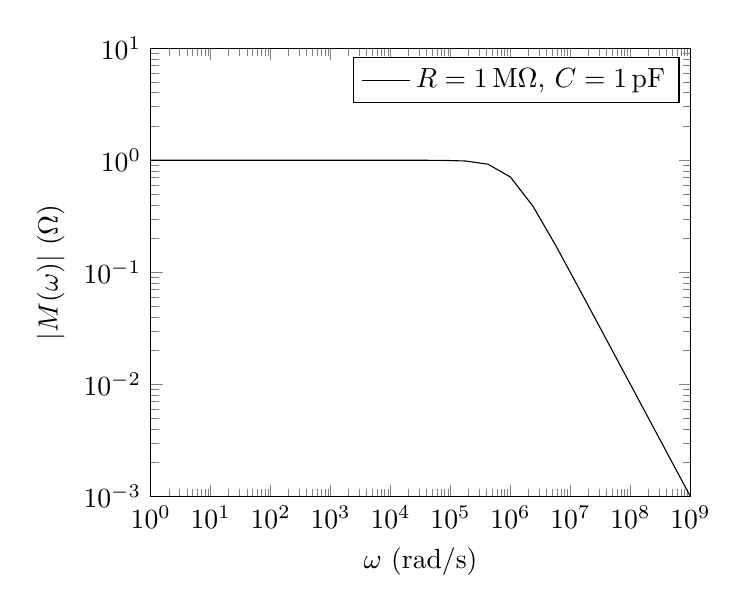
\begin{tikzpicture}
\begin{loglogaxis}[
    xlabel=$\omega$ (\SI{}{\radian / \second}), ylabel=$\abs{M(\omega)}$ (\SI{}{\ohm}),
    xmin=1, xmax=10^9,
    ymin=10^(-3), ymax=10,
    % legend style={at={(0.02,0.98)},anchor=north west},
 ]
\addplot [domain=1:1000000000] {1/sqrt(1 + x^2 / 10^12)};
\addlegendentry{$R = \SI{1}{\mega\ohm}$, $C = \SI{1}{\pico\farad}$}
\end{loglogaxis}
\end{tikzpicture}
\end{center}

This graph should look very familiar from previous lectures. Note that for low values of $\omega$, the capacitor acts like an open circuit, so there is very little voltage drop, whereas at high values of $\omega$, the capacitor acts more like a short, and the output voltage drops rapidly. Making this more precise, we will consider two cases:
\begin{itemize}
    \item Case 1: $\omega \ll 1 / (RC)$. Note that this implies that $\omega RC \ll 1$. In this case,
    \eqn{
        && M(\omega) &= \frac{1}{\sqrt{1 + \omega^2R^2C^2}} \\
        &&&\approx \frac{1}{\sqrt{1}} \\
        &&&= 1.
    }
    Thus, for small values of $\omega$, our output voltage will have practically the same magnitude as the input.
    \item Case 2: $\omega \gg 1 / (RC)$. Note that this implies that $\omega RC \gg 1$. In this case,
    \eqn{
        && M(\omega) &= \frac{1}{\sqrt{1 + \omega^2R^2C^2}} \\
        &&&\approx \frac{1}{\sqrt{\omega^2R^2C^2}} \\
        &&&= \frac{1}{\omega R C}.
    }
    Taking logs of both sides to compute the behavior on a log-log plot,
    \eqn{
        && \log{(M(\omega))} &\approx \log{\left(\frac{1}{\omega RC}\right)} \\
        &&&= -\log{(RC)} - \log{(\omega)},
    }
    giving us a straight line with a slope of negative unity.
\end{itemize}
Plotting both of these approximations along with the actual result, we obtain
\begin{center}
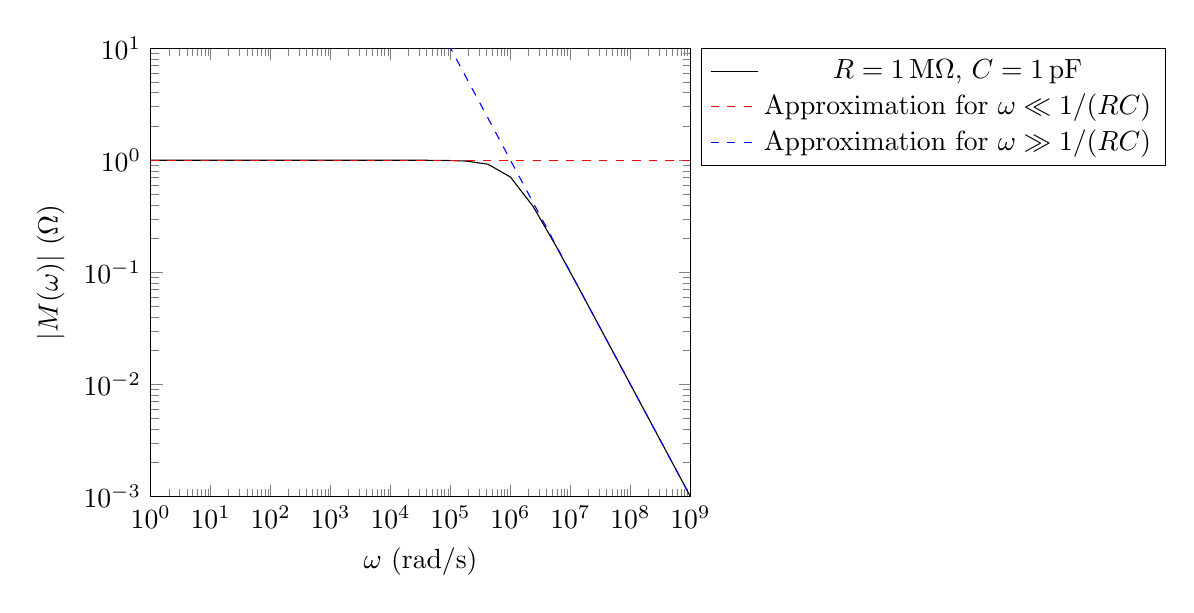
\begin{tikzpicture}
\begin{loglogaxis}[
    xlabel=$\omega$ (\SI{}{\radian / \second}), ylabel=$\abs{M(\omega)}$ (\SI{}{\ohm}),
    xmin=1, xmax=10^9,
    ymin=10^(-3), ymax=10,
    legend style={at={(1.02,1)},anchor=north west},
 ]
\addplot [domain=1:1000000000] {1/sqrt(1 + x^2 / 10^12)};
\addplot [domain=1:1000000000, color=red, dashed] {1};
\addplot [domain=1:1000000000, color=blue, dashed] {1 / (x * 10^6 * 10^(-12))};
\addlegendentry{$R = \SI{1}{\mega\ohm}$, $C = \SI{1}{\pico\farad}$}
\addlegendentry{Approximation for $\omega \ll 1 / (RC)$}
\addlegendentry{Approximation for $\omega \gg 1 / (RC)$}
\end{loglogaxis}
\end{tikzpicture}
\end{center}

Note that the intersection of our two approximations occurs at $\omega = 1 / (RC)$.

We may also plot $\theta$ on a log plot. Note that while we will plot $\omega$ on a log-scale, we will plot the phase shift $\theta$ itself on a linear scale, since it only varies within a small range of values:
\begin{center}
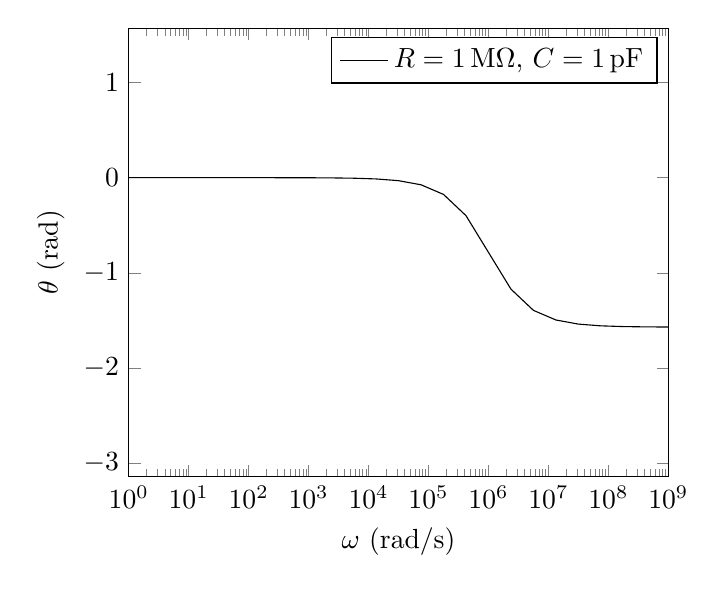
\begin{tikzpicture}
\begin{semilogxaxis}[
    xlabel=$\omega$ (\SI{}{\radian / \second}), ylabel=$\theta$ (\SI{}{\radian}),
    xmin=1, xmax=10^9,
    ymin=-pi, ymax=pi / 2,
    % legend style={at={(1.02,1)},anchor=north west},
 ]
\addplot [domain=1:1000000000] {(-pi / 180) * atan(x * 10^6 * 10^(-12))};
\addlegendentry{$R = \SI{1}{\mega\ohm}$, $C = \SI{1}{\pico\farad}$};
\end{semilogxaxis}
\end{tikzpicture}
\end{center}

Putting the plots of $M(\omega)$ (on a log-log scale) and $\theta$ together, we obtain what is known as a \emph{Bode plot}. We will discuss these plots more in upcoming lectures.


\end{document}
